\chapter{Statistics of the South Flood-North Drought: A new catalog of rainbands in the East Asian monsoon}

%consider uploading your actual code to this chapter for reproducibility.

\section{Abstract}
A novel 57-year (1951-2007) daily catalog of frontal rainbands over China is compiled based on APHRODITE rain gauge data, resulting in an unprecedented climatology of Meiyu front progression in summer. Late \nth{20}-century changes in Chinese summer rainfall are investigated (the ``South Flood-North Drought''). Two robust changes in front behavior are observed during 1980-2007 relative to 1951-1979: 1) A significant decrease in the frequency of frontal rainbands during the Pre-Meiyu period (May), and 2) a southward shift in Post-Meiyu rainbands (mid-July to September). In contrast, the years 1994-2007 are marked by an increase in frontal intensity during Meiyu season relative to 1979-1993, but not frequency. By finding changes in the component of China rainfall associated with the large-scale atmosphere, our results begin to address the critical question of whether the South Flood-North Drought will persist under \nth{21}-century global warming.

%Changes in rainfall can be traced to changes either in the frequency of events, or in their mean intensity. However, according to \cite{Biasutti2011}, the instantaneous strength of rainfall does not change with time - therefore, long-term changes can be traced to changes in frequency.

\section{Introduction}

 	Eastern China receives about 60\% of its rainfall from May to August via the East Asian summer monsoon. The period of peak rainfall lasting from early June to mid-July is called ``Meiyu season'' (lit. ``plum rains,'' referring to the spectacular growth of plum blossoms in central China with the onset of heavy rains). During this time, heavy rainfall occurs in zonal bands resulting from frontal synoptic conditions (the ``Meiyu front''). The rainfall climatology of Japan and Korea also features similar phenomena known as Baiu and Changma respectively. A growing volume of evidence suggests a shift in rainfall over China beginning in the late 1970s, featuring a ``South Flood-North Drought'' pattern shown in Figure \ref{changes_2d}a \citep{Hu1997,Gong2002,Nigam2013}. Due to the severe human impacts of the South Flood-North Drought on densely-populated eastern China, it is vital to understand whether this pattern will strengthen under global warming, or represents only a temporary deviation from the mean.
 
	The climatology of the East Asian monsoon bears little resemblance to other monsoon circulations \citep{Ding2005}. Whereas understanding of tropical monsoons has progressed greatly via theoretical studies \citep{Plumb1992,Prive2007,Bordoni2008}, the dynamics that favor the existence of frontal convection over East Asia in summer remain a point of debate, centering around the interplay of the tropospheric jet and Tibetan Plateau \citep{Molnar2010,Sampe2010,Chen2014}. Therefore, no simple conceptual template exists for interpreting a change such as the South Flood-North Drought. However, it is known that the migration of the Meiyu front entails a series of large-scale circulation changes \citep{Chen2004}, and furthermore that anomalies in Meiyu front latitude produce corresponding rainfall anomalies \citep{Kosaka2011}. Therefore, the South Flood-North Drought should be describable in terms of changes in the properties of Meiyu rainbands, such as a shift in latitude, a change in intensity or an earlier or delayed northward migration. In turn, such a characterization may provide insight into the dynamics responsible for the change.
	
	In pursuit of this aim, we have developed a 57-year database (1951-2007) of frontal rainbands in China based on the APHRODITE rain gauge product (described below). We develop a recursive convergent fitting algorithm of daily rainfall maps which finds rainbands and quantifies their attributes. Previous studies have investigated the statistics of the Meiyu front on decadal and even centennial timescales \citep{Chen2004,Ge2008,Xu2009}, but to our knowledge no previous author has compiled a multi-decadal daily catalog of events. We use this catalog to clarify the spatial and temporal attributes of the South Flood-North Drought, and present it as a tool for future East Asian monsoon research. We also expect that the South Flood-North Drought corresponds to larger-scale late-twentieth-century climatic changes, in particular the tropospheric jet, which plays an essential and complex role in East Asian summer climate \citep{Molnar2010}. We propose that changes in the timing of East Asian tropospheric jet migrations induced observed twentieth-century changes in China rainfall. This hypothesis is described below, and will be further explored in future work.

\section{APHRODITE}

Can probably remove subsection since previously described in thesis.

	\textcolor{blue}{The APHRO\_MA\_V1101 product from APHRODITE (Asian Precipitation - Highly-Resolved Observational Data Integration Towards Evaluation of the Water Resources) includes 57 years (1951-2007) of daily rainfall (PRECIP product) on a .25\$^{\circ}$\ $\times$ .25\$^{\circ}$\ grid over 60-150\$^{\circ}$ E and 15\$^{\circ}$ S-55\$^{\circ}$ N \citep{Yatagai2012}. Values are assimilated from weather station observations and therefore available over land only. We focus on the subregion inside of 100\$^{\circ}$ E-123\$^{\circ}$ E and 20\$^{\circ}$ N-40\$^{\circ}$ N, where Meiyu rainbands occur. Stations in this region are spaced at 100-200 km intervals (shown by RSTN product), such that rainbands are clearly resolved. APHRODITE's resolution cannot capture some features visible in TRMM satellite data \citep{Xu2009}, but its length allows for the study of decadal change.}
	
\section{Rainband Detection Algorithm}

\subsection{Overview}

	For each day from 1 January 1951 to 31 December 2007 (20,819 days total), our recursive convergent image processing algorithm determines whether a rainband, defined as a continuous chain of rainfall maxima exceeding 10 mm day$^{-1}$ spanning at least 5\$^{\circ}$ of longitude, exists inside the window of 105-123\$^{\circ}$ E and 20-40\$^{\circ}$ N. Properties of the rainband are calculated including latitude, intensity, tilt, length and width, as well as a ``quality score'' $Q$, defined as the fraction of daily rainfall occurring within the band. Fits with $Q<.6$ are discarded. We also test for the existence of two rainbands on a single day, an arrangement commonly found in August and September. In such a case, the first and second fitted rainbands are referred to as ``primary'' and ``secondary'' rainbands respectively. Our algorithm does not distinguish between the mechanisms that supply rainfall. Metrics of algorithm performance are documented in Supplementary Tables S1-S3. 
	
\subsection{Recursive Convergent Image Processing}

\begin{enumerate}
	\item Given a map of daily accumulated rainfall over the longitudes 105-123$^{\circ}$E and 20-40$^{\circ}$N at $.25^{\circ}$ by $.25^{\circ}$ resolution, the daily rainfall maximum at each longitude is found, and its intensity and latitude recorded. If there exists a $5^{\circ}$ continuous chain of maxima (20 points in a row) exceeding 10 mm day$^{-1}$, we proceed to step 2 and attempt a fit (Figure S1a). Otherwise, no fit is attempted for that day (Figure S1b).
	
	\item In order to approximate the position of the rainband with a best fit line, a weighted least-squares linear fit of the \textit{latitudes} of the maxima is performed in MATLAB using the intensity of each maximum as weight. To encourage convergence, the weight of outlying points is set to zero, where an outlier is defined as any maximum that is over $5^{\circ}$ from the centroid of the precipitation maxima $\left<lat_{max}\right>$, calculated by $\left<lat_{max}\right>=\frac{\sum_{long} lat_{max}*max}{\sum_{long} \max}$.
	
	\item A recursive algorithm converges on a best estimate of rainband position. In each iteration, we find a new set of maxima within \textit{k} degrees of the previous best fit line, and again perform a weighted linear fit of the maxima (Figure S2a). $k$ is progressively decreased with each iteration from $5^{\circ}$ to $2^{\circ}$ by $.25^{\circ}$ increments, and then from $2^{\circ}$ to $.25^{\circ}$ by $.25^{\circ}$ increments but repeating each width $k$ twice in a row (Figures S2b-c). The fit obtained in the final iteration is taken as our best estimate (Figure S2d).
	
	\item We define the ``quality score'' $Q$ as the fraction of total daily precipitation inside of  that falls within $2.5^{\circ}$ degrees of the best estimate line (Figure 4b). Other rainband properties are calculated as follows. Rainband latitude is defined as the latitude of our fitted band at the reference longitude of 115$^{\circ}$E. Intensity is defined as mean rainfall at all points along the band axis where daily rainfall exceeds 5 mm day$^{-1}$ (``rainband points''), length as the total number of rainband points (expressed in units of degrees of longitude), and width as the mean distance between half-maxima on either side of each rainband point (units of degrees of latitude).
	
	\item Given an estimate of primary rainband, we check for a secondary rainband. We start by removing all precipitation associated with the primary rainband from our daily rainfall map. To do this, all rainfall within 4$^{\circ}$ of our primary rainband is set to 0, as well as rainfall at any other adjacent points where rainfall exceeds 10 mm day$^{-1}$ (Figure S3a). We then reapply the continuous maximum criterion from step 1 (Figure S3b). If passed, steps 2-4 are repeated to find a best estimate for the position of the secondary rainband, and its attributes calculated.
	
	\item If a secondary rainband is found, two additional quality scores $Q_1$ and $Q_2$ are calculated. $Q_1$ is defined as the fraction of daily rainfall inside of 105-123$^{\circ}$E and 20-40$^{\circ}$N that is contained within $2.5^{\circ}$ degrees of the primary rainband \textit{after removing all rainfall associated with the secondary rainband} (equivalently, the $Q$ score after removing the secondary rainband). Likewise, $Q_2$ is the $Q$ score of the second rainband \textit{after removing all rainfall from the primary rainband} (Figure S4d).		
	
\end{enumerate} 

In rare cases with two rainbands of roughly equal strength but well-separated in latitude, the removal of outliers in step 2 prevents a fit entirely. We test for such cases by ensuring that the total sum of weights ${\sum_{long} max}$ exceeds 200 mm day$^{-1}$, equivalent to our condition in bullet point 1. When this condition is failed, which can only occur when too many of our maxima have been discarded, we return to step 1, but find maxima only over the latitude range 20N-$\left<lat_{max}\right>$ or $\left<lat_{max}\right>$-40N, depending on which half of our domain has a longer chain of maxima exceeding 10 mm day$^{-1}$, and apply the remaining steps of our algorithm as usual.

\subsection{Quality Control}

After running the algorithm for all 20,819 days from 1 January 1951 to 31 December 2007, we obtained 11,228 days with at least one rainband and 1,116 days with two rainbands. Subsequently, we apply a quality control (QC) algorithm to eliminate days with poor fit, based on the quality scores $Q$, $Q_1$ and $Q_2$ as well as the ``Taiwan fraction'' (TW), defined as the percentage of daily rainfall inside the window 105-$123^{\circ}$E and 20-$40^{\circ}$N that falls over the island of Taiwan (roughly 120-$122^{\circ}$E and 22-$26^{\circ}$N. We use these metrics to define the following two criteria for inclusion:

\begin{enumerate}

	\item If $TW > 20\%$, the day's fit is thrown out (238 cases total, 2.1\% of total fits). Such days are dominated by a local storm reaching Taiwan and do not exhibit a strong rainband (Figure 4a).  
	
	\item Subsequently, a day can be included if it meets either of the following criteria:
	
	\begin{enumerate} 
	
	\item if $Q>.6$, the day is included in our statistics (7,522 days, 67.0\% of total fits; Figure 4b). If $Q_2$ is also greater than .6, the day will be classified as a double rainband day (Type I double rainband; 232 cases, or 3.1\% of days where $Q>.6$ and $Q_2>.6$).
		
	\item If $Q<.6$, the day is discarded unless two fronts are detected and both $Q_1 \mathrm{\textbf{ and }} Q_2 > .6$ (where again $Q_1$ and $Q_2$ are \textit{conditional} quality scores as defined above). In such cases, the presence of multiple rainbands of similar intensity initially obscures the quality of the fit (Figure 4d). Such days are also classified as double rainband days (Type II double rainband; 466 cases). In the absence of such a double rainband configuration the day is thrown out (Figure 4c).
	
	\end{enumerate}
	
\end{enumerate}	

	The use of conditional quality scores $Q_1$ and $Q_2$ adds 466 double rainband days that would otherwise have been categorized as days with no rainband, constituting 6.2\% of total days included in our statistics. 33.2\% of double rainband days are Type I ($Q>.6$) and 66.8\% Type II ($Q<.6$). Double rainbands are more common during certain seasons. Tables \ref{t51}-\ref{t53} contain more information on algorithm functionality. 

%%% TABLE 5.1 - ALGORITHM FUNCTIONALITY - BIG PICTURE	
\begin{table}

\caption{Statistics on the functionality of the rainband detection algorithm. Number in parentheses indicates the percentage of days that fall into that category out of all 20,819 days.}
\centering

\begin{tabular}{ l c c c}
	  & Total Fits & Passes Quality Control & Percent Passing QC\\
	 \hline
	 Primary rainband found & 11,228 (53.9\% of total) & 7,988 (38.4\% of total) & 71.1\% \\
	 Secondary rainband found & 1,116 (5.4\% of total) & 698 (3.4\% of total) & 62.5\% \\
\end{tabular}
\label{t51}
\end{table}

%%% TABLE 5.2 - ALGORITHM FUNCTIONALITY - DETAILS, PRIMARY RAINBAND
\begin{table}

\caption{Details on the application of quality control (QC) criteria to primary rainbands.}
\centering

\begin{tabular}{ l c}
	 Criterion & Number (\% of total) \\
	 \hline
	 Primary rainband days before QC & 11,228 \\
	 Taiwan days (TW$>20\%$) & 238 (2.1\%) \\
	 $Q>.6$ (strong rainband) & 7,522 (67.0\%) \\
	 Double rainband ($Q_1>.6$ and $Q_2>.6$) & 466 (4.2\%) \\
	 Poor fit (Fails QC) & 3008 (26.8\%) \\
	 
\end{tabular}
\label{t52}
\end{table}

%%% TABLE 5.3 - ALGORITHM FUNCTIONALITY - DETAILS, SECONDARY RAINBAND
\begin{table}

\caption{Details on the application of quality control (QC) criteria to secondary rainbands. Type I and Type II fits are defined in supplementary text above.}
\centering

\begin{tabular}{ l c}
	 Criterion & Number (\% of total) \\
	 \hline
	 Secondary rainband days before QC & 1,116 \\
	 Type I fit ($Q>.6$ and $Q_2>.6$) & 232 (20.8\%) \\
	 Type II fit ($Q_1>.6$ and $Q_2>.6$) & 466 (41.8\%) \\
	 Poor fit (Fails QC) & 418 (37.5\%) \\
	 
\end{tabular}
\label{t53}
\end{table}

%%EXPLANATORY FIGURES SHOWING ALGORITHM FUNCTIONALITY

%5.1 - displaying continuous maximum criterion required to attempt rainband fit
\begin{figure}

\noindent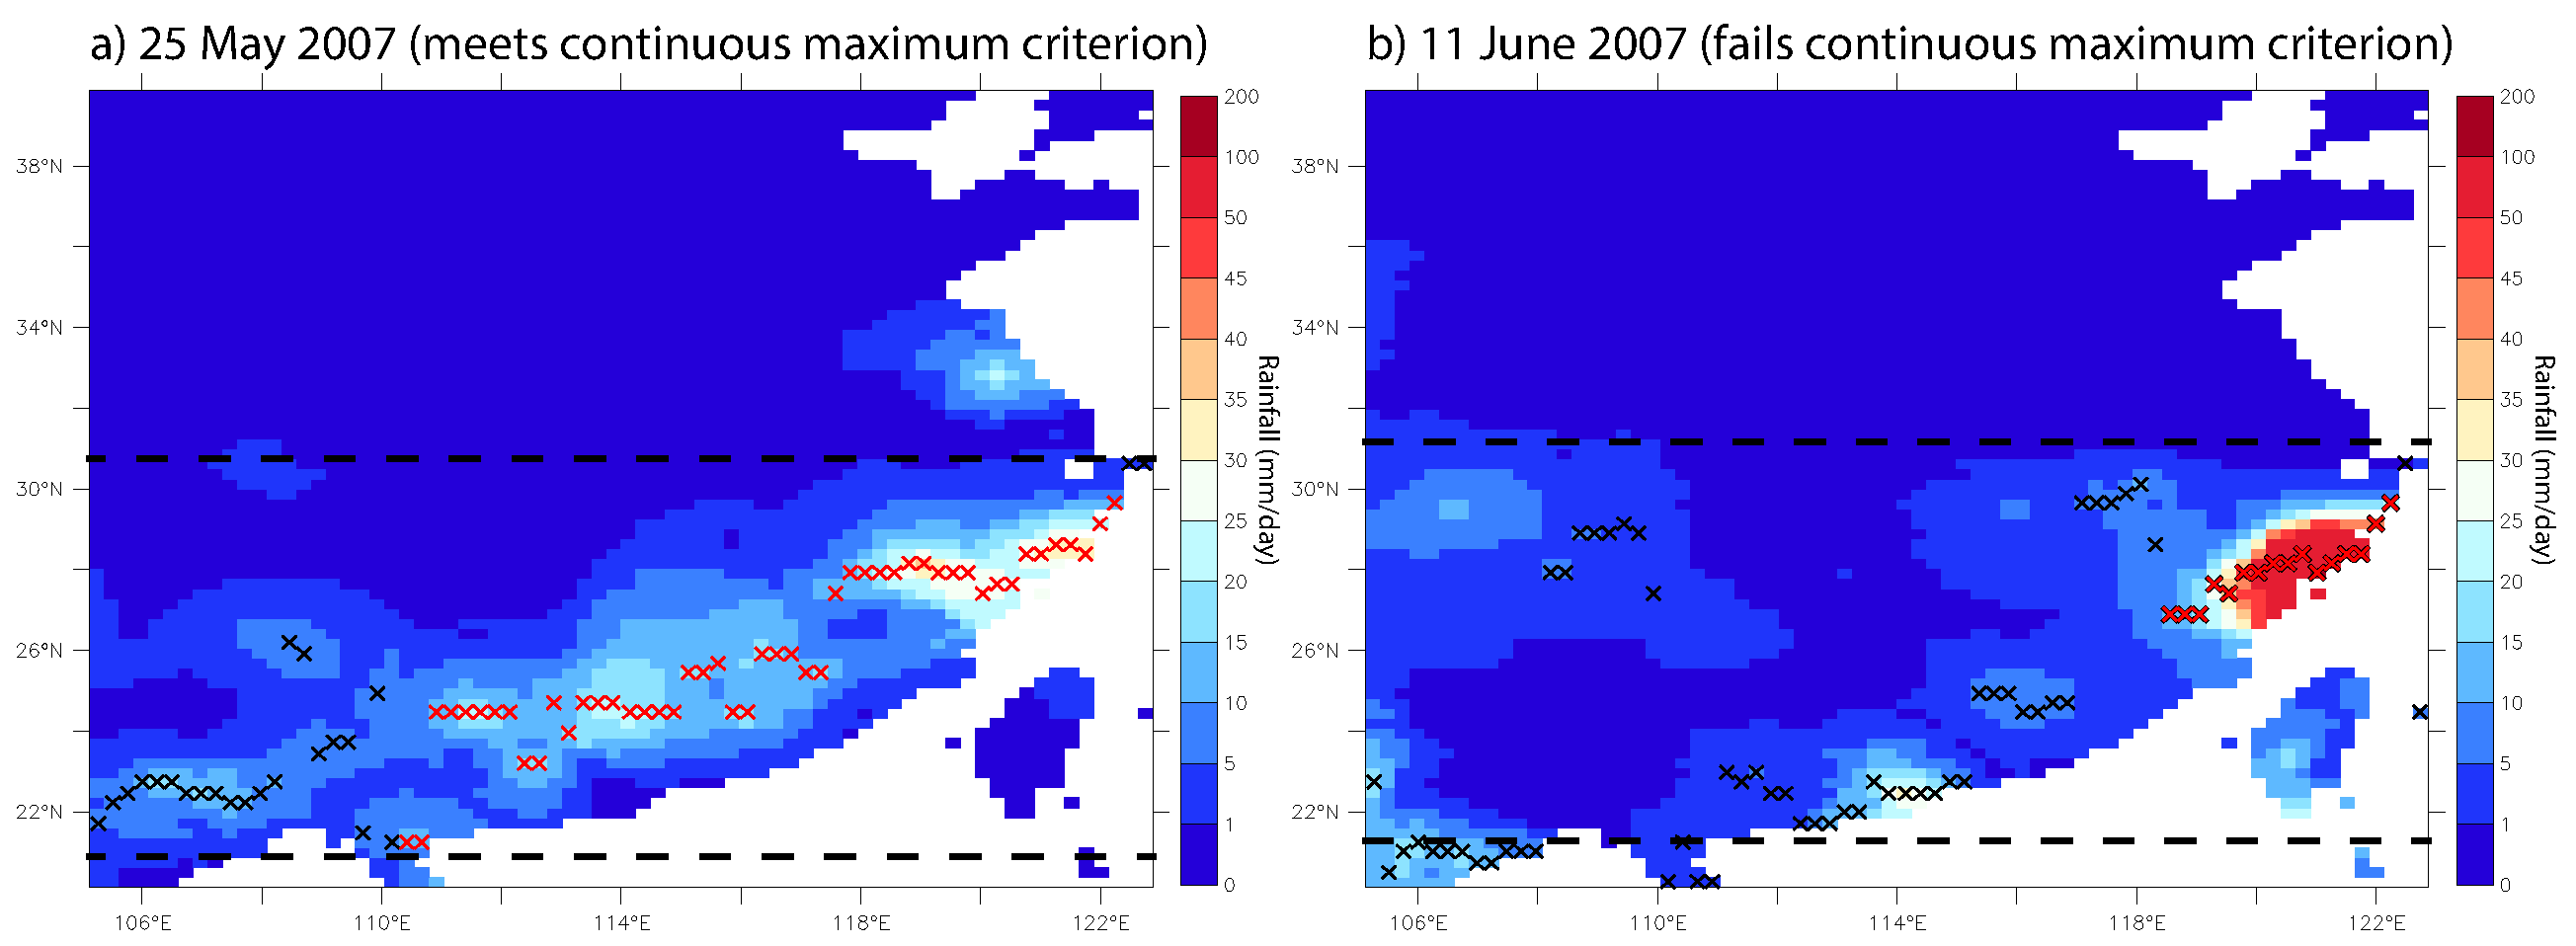
\includegraphics[width=36pc]{S1}
\caption{The first step of the rainband detection algorithm checks to see whether a five-degree continuous longitudinal band of precipitation maxima above 10 mm day$^{-1}$ exists. If so, a rainband fit is attempted. a) 25 May 2007 - the continuous maximum criterion is met and a fit is attempted. b) 11 June 2007 - although there is abundant rainfall in some locations, it appears not to be frontal and the continuous maximum criterion is failed. No fit is attempted.}
\label{f51}
\end{figure}

%5.2 - How the convergent fit algorithm works.
\begin{figure}

\noindent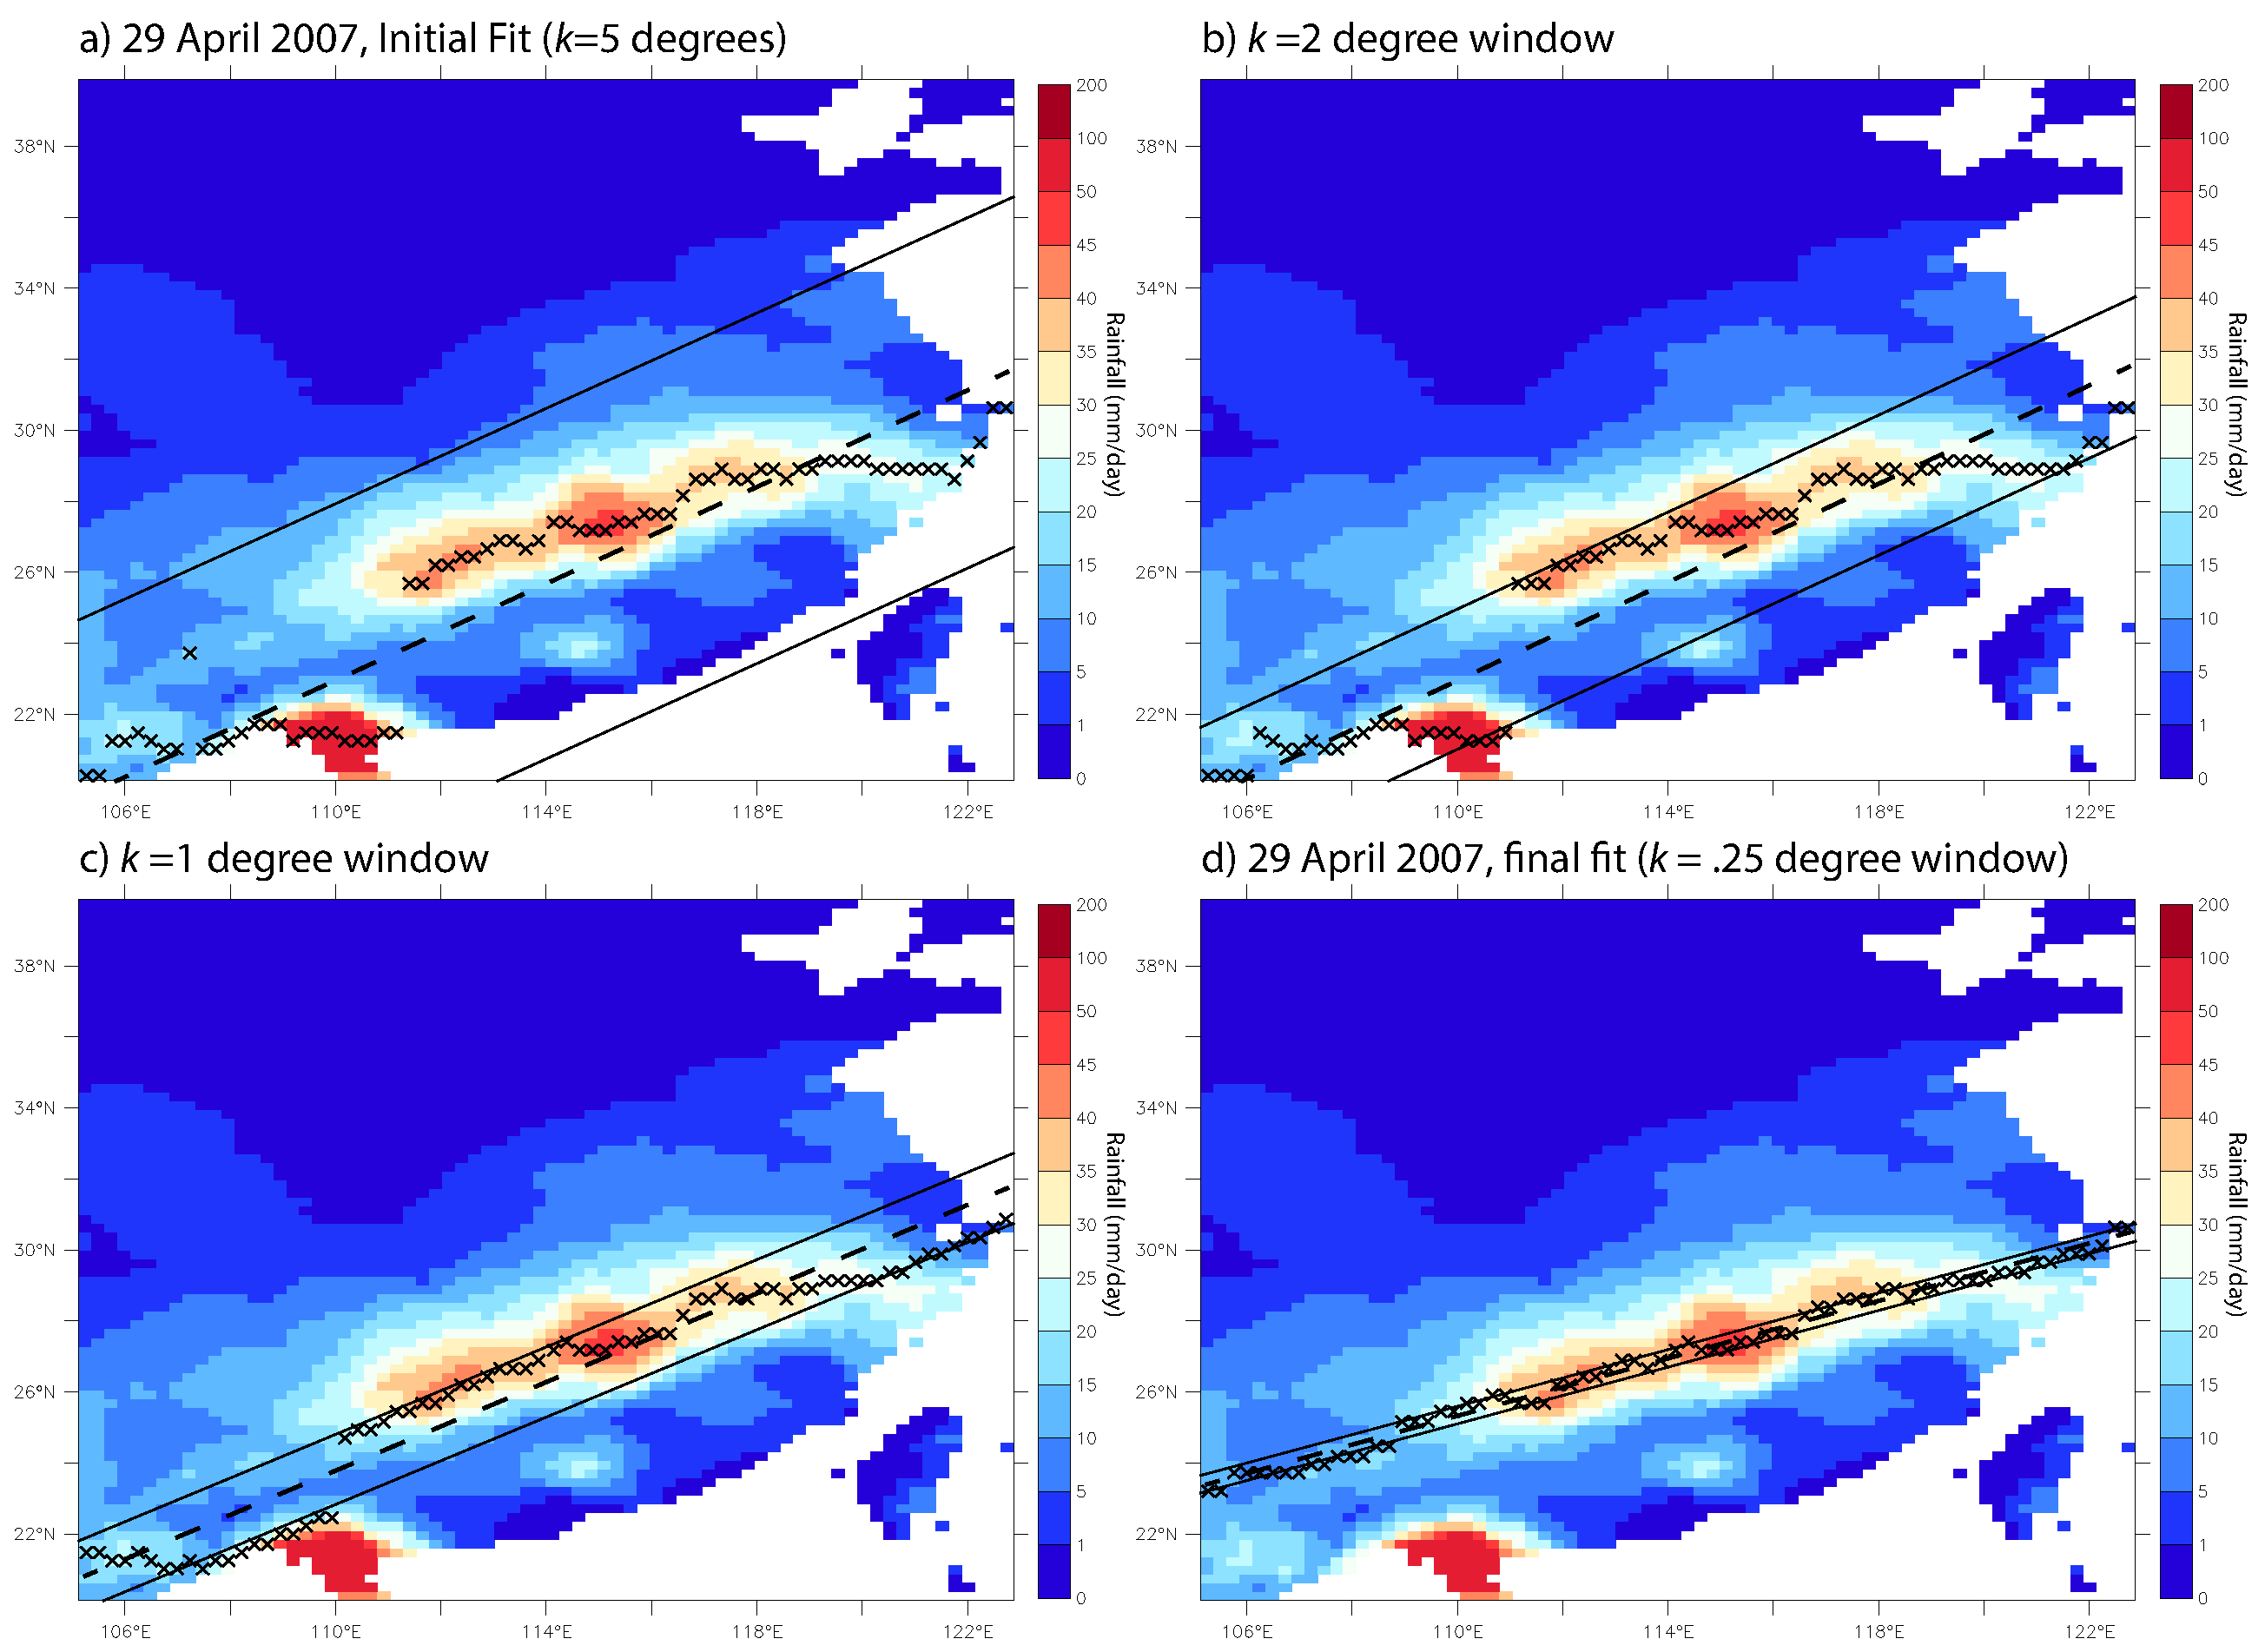
\includegraphics[width=36pc]{S2}
\caption{Display of the functionality of the recursive convergent algorithm. On 29 April 2007, a strong maximum in southernmost China skews our initial rainband fit (a), but the algorithm eventually converges on the most prominent coherent band via tighter windowing (d).}
\label{f52}
\end{figure}

%5.3 - Procedure for finding double rainbands
\begin{figure}

\noindent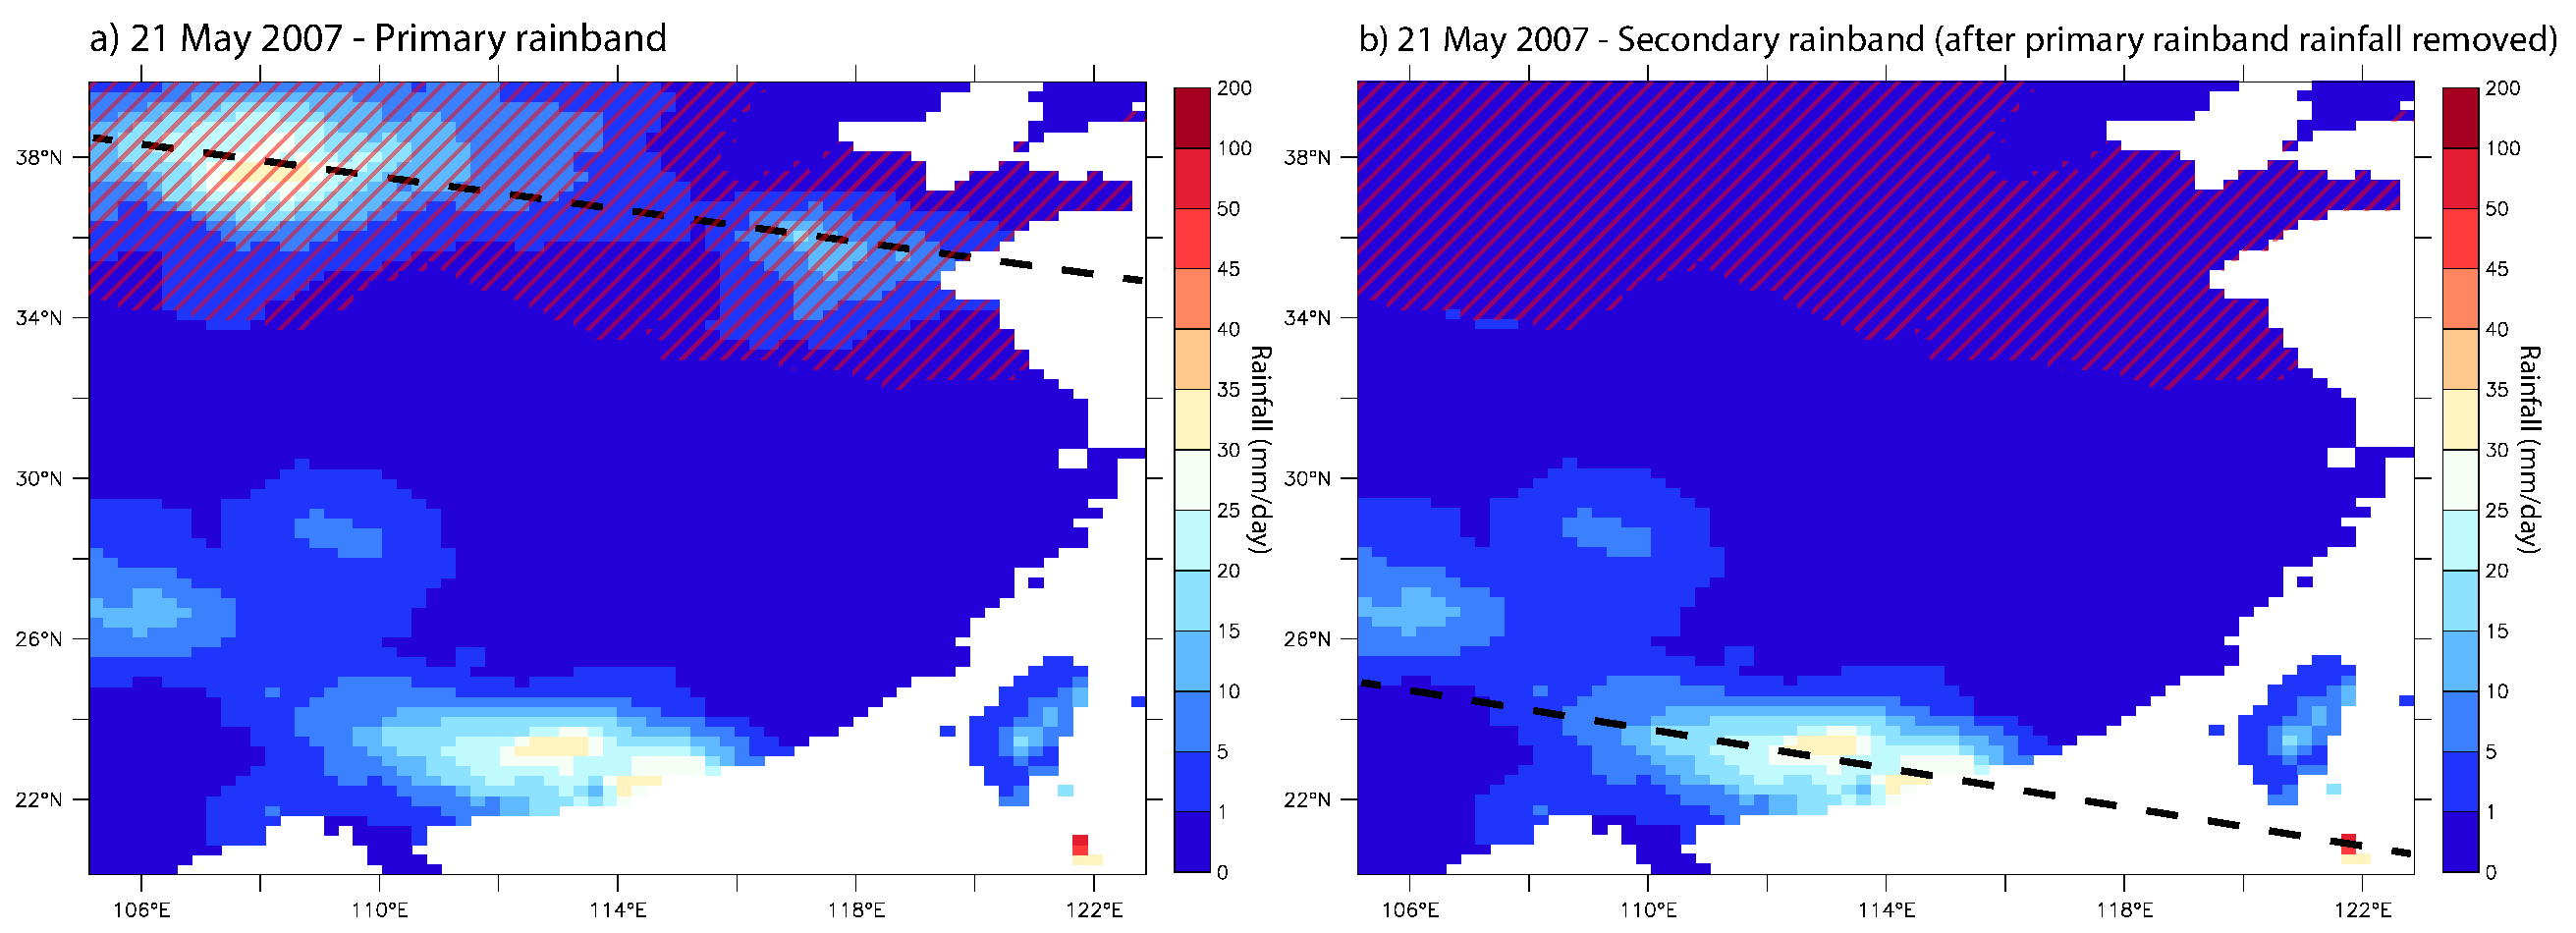
\includegraphics[width=36pc]{S3}
\caption{a) The algorithm converges on the strongest rainband, around 37N (defined as the ``primary rainband''). b) The rainfall associated with the primary rainband is removed, and we check for the presence of another rainband (a ``secondary rainband''), again using the continuous maximum criterion.}
\label{f53}
\end{figure}

%5.4 - Quality Control algorithm used to determine inclusion in statistics
\begin{figure}

\noindent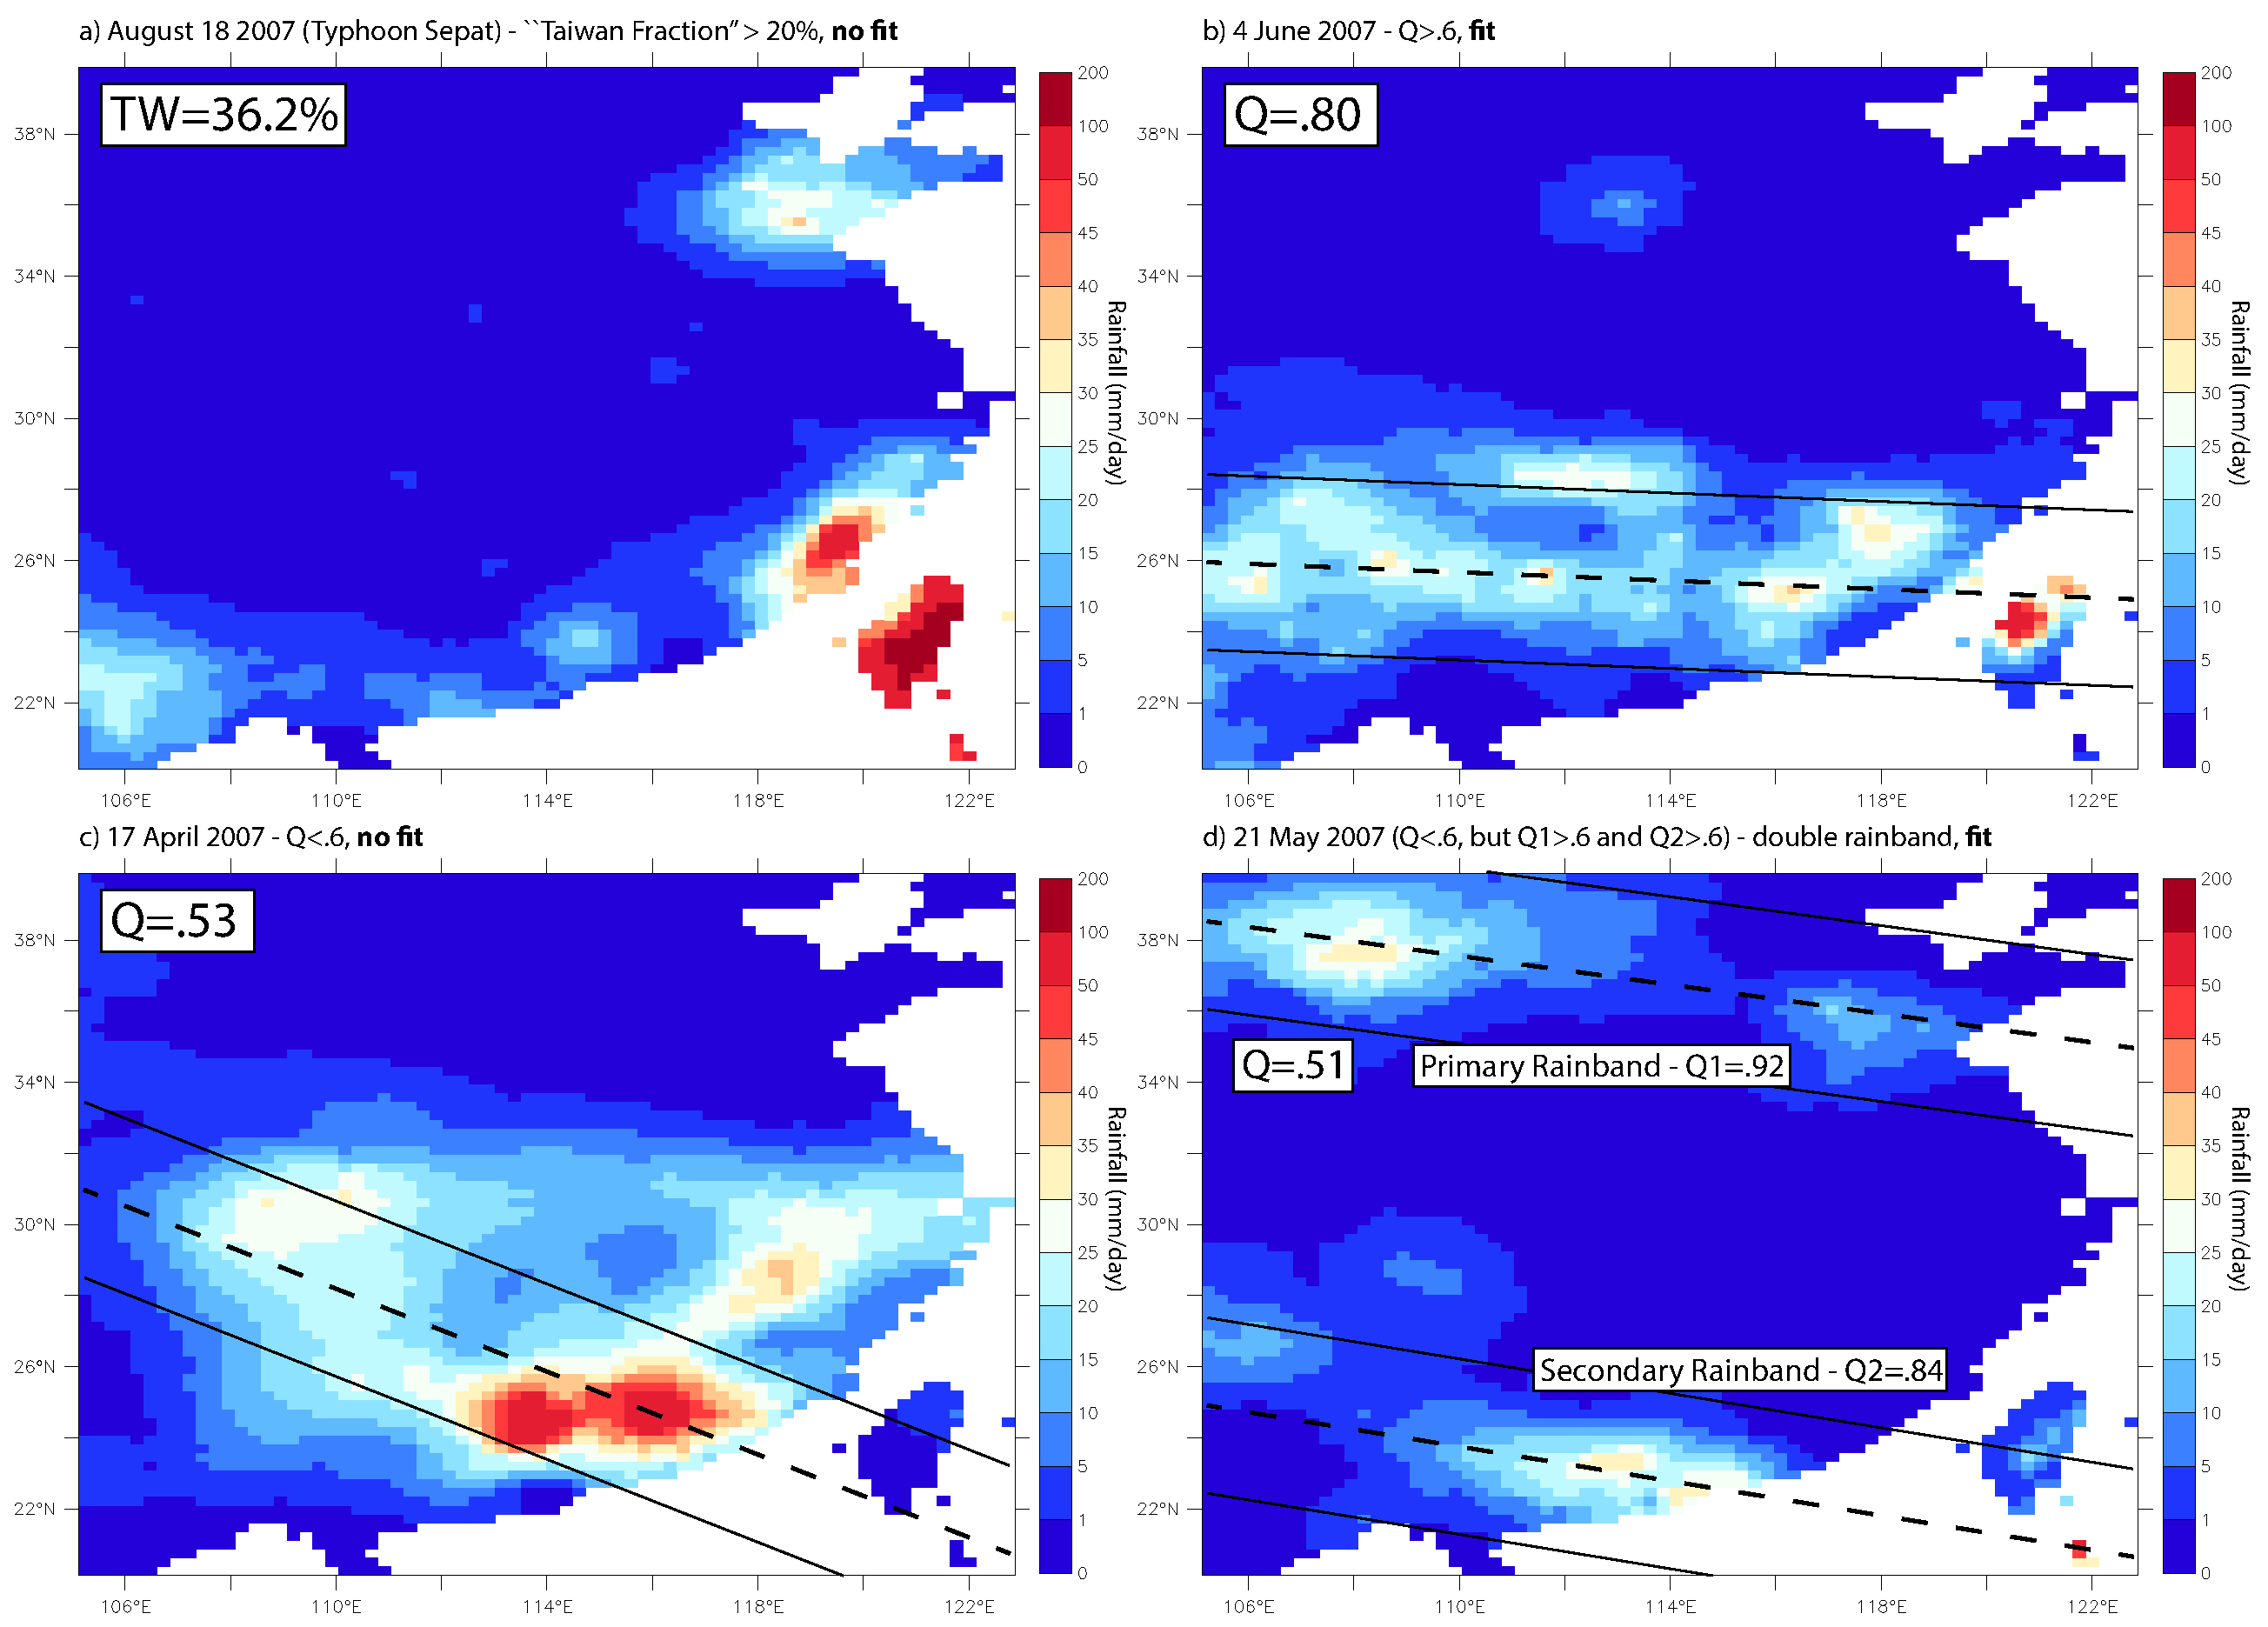
\includegraphics[width=36pc]{S4}
\caption{A quality control algorithm is used to exclude poor fits. a) 18 August 2007 - Days with a high Taiwan fraction (here, corresponding to the passage of Typhoon Sepat) are excluded from our statistics. b) June 4 2007 - A high-quality fit is achieved. c) 17 April 2007 - Although a fit is reached, it explains the distribution of daily rainfall poorly and is therefore excluded from rainband statistics. d) 21 May 2007 (same day as Figure S3) - An initial fit appears to be of poor quality ($Q<.6$). However, after finding a secondary rainband, we determine that conditional quality scores $Q_1$ and $Q_2$ are high, and the day is included in our statistics.}
\label{f54}
\end{figure}


%% BOOTSTRAPPING
\subsection{Significance of Changes - Bootstrapping Algorithms}

	The standard deviation and significance of changes in rainband frequency are calculated analytically. However, the distribution of rainband latitude and intensity during a given season is not constrained to follow a normal distribution (INSERT CITATION ABOUT USE OF GAMMA DISTRIBUTION?). Therefore, in the estimation of statistical significance we are required to employ non-parametric tests. In this chapter, estimations of significance were obtained using bootstrapping with and without replacement (the latter also known as a permutation method), well-established techniques that allow the estimation of relevant quantities by constructing synthetic distributions \citep{Good2005}.
	
	Furthermore, rainband statistics are not independent from one day to the next, but rather exhibit temporal autocorrelation greater than 1. Intuitively from our knowledge of weather, the observation of a front at a particular latitude makes it more likely that it will be subsequently observed at the same latitude. We employ a technique known as a \textit{moving blocks bootstrap}, described for instance in citep{Singh}. In this case, data are drawn in sequential blocks of $n$ days depending on the strength of the temporal autocorrelation. The choice of block length $n$ is a subject of substantial debate in the statistical literature, but in practice, the choice of block length ranging from 2 to 5 days does not substantially alter our estimations of statistical significance, although in general the choice of longer blocks tends to return the estimated p-value closer to .5.
	
	In our case, we face the added problem that not all variables are continuous in time. If no front is observed on a day then we cannot report a latitude or intensity. In testing the significance of changes in front latitude and intensity, we have relied on a regular permutation test, because there is no existing convention to our knowledge for handling the case of missing observations in a moving blocks bootstrap. We rely on alternative methods such as the Anderson-Darling and Kolmogorov-Smirnov tests to further gauge the magnitude of such changes.
	
	We use bootstrapping with replacement to calculate the standard deviation of their means (Figure \ref{jet_seasonal}a and Supplementary Tables S4-S8 respectively). Both bootstrapping with replacement and a permutation test produce similar results; $p$-values shown are from permutation testing. Figure 3a uses a moving blocks bootstrap with block length of 3 days (Supplementary Text S3). We focus on changes in front attributes between 1951-1979 and 1980-2007 (Supplementary Tables S5 and S6), and also repeat our methodology for 1979-1993 versus 1994-2007, since other authors have found a significant shift between these sets of years.

	Below we attach the relevant code used to perform bootstrapping with replacement, without replacement (permutation test) and the moving blocks bootstrap.

...%code



\section{Results}

\subsection{Comparison with alternative metrics}
It is reasonable to suggest that some simpler metric ought to exist that reproduces the results of the Rainband Detection Algorithm (RDA). In this section, we test a suite of simple metrics, using the same bootstrapping algorithms used to calculate the statistical significance of changes in observed yearly rainfall. These metrics are as follows: ...

The following figure demonstrates the climatology of the 8 metrics described above:

\begin{figure}[htb]

\noindent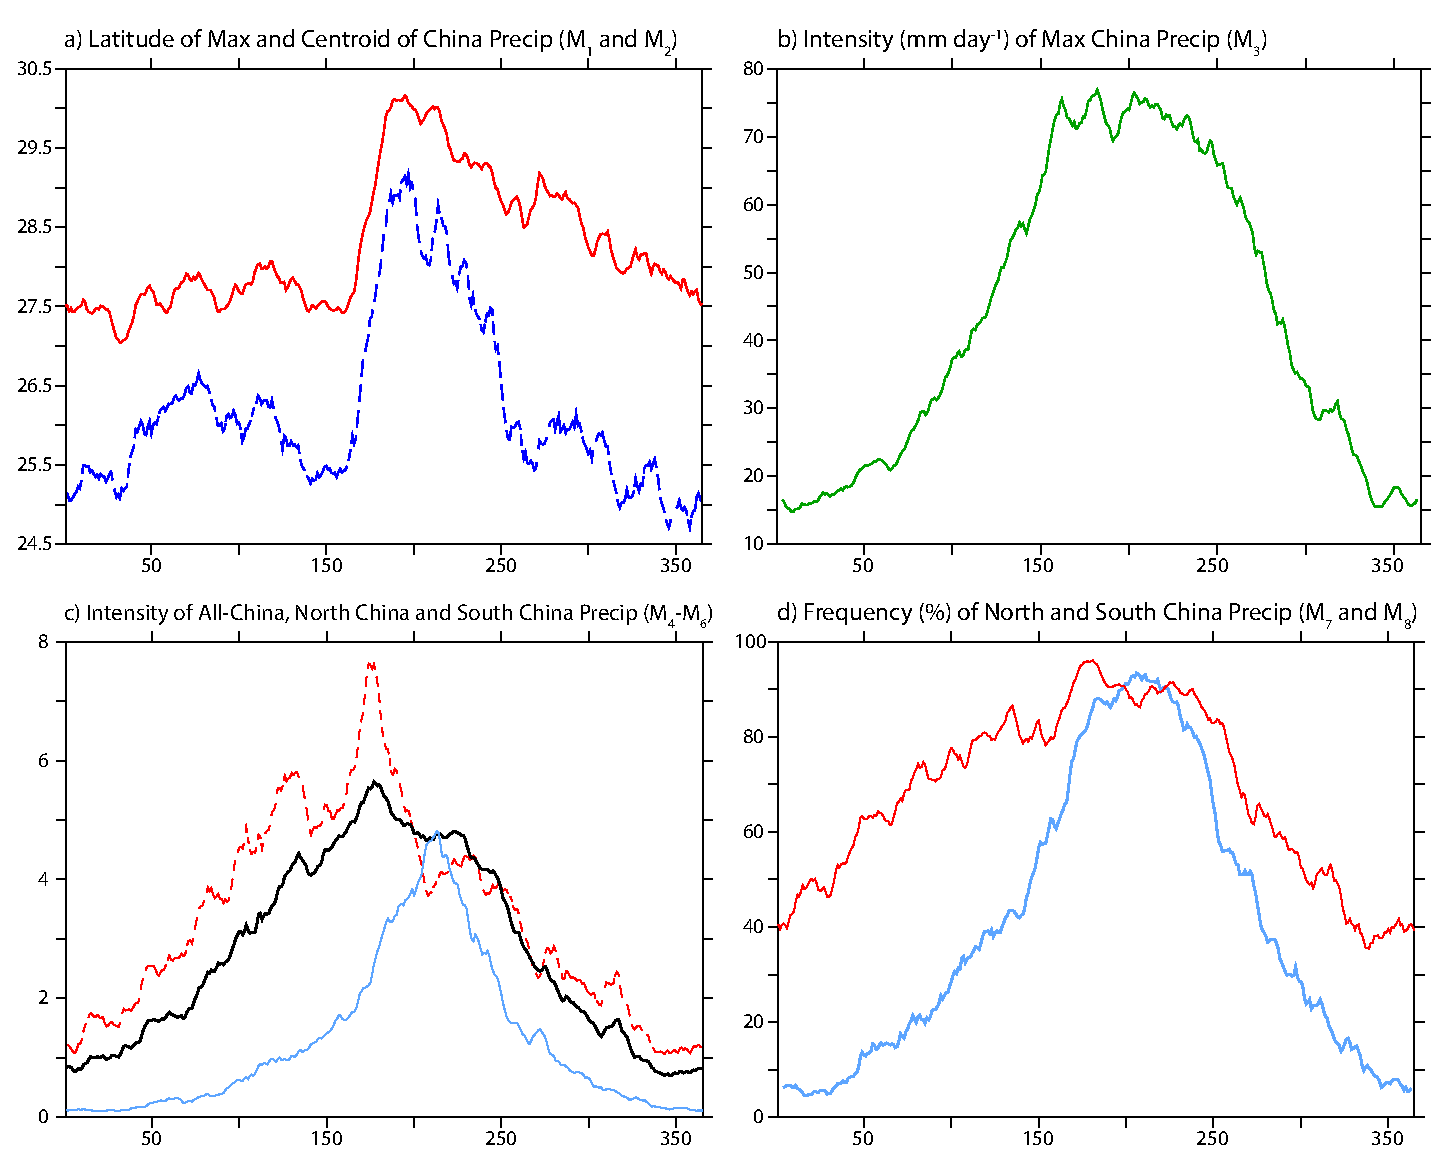
\includegraphics[width=36pc]{Figures/A3_met_climo}
\caption{1980-2007 versus 1951-1979 changes in frontal and local rainfall for full year (a and b), Pre-Meiyu (c and d) and Post-Meiyu (e and f)}
\end{figure}



%%%% ALTERNATIVE METRIC STATISTICS, 1951-1979 %%%%
\begin{table}[p]

\centering

\caption{Mean and standard deviation of mean of metrics $M_1$ to $M_8$ for 1951-1979 as previously defined. Standard deviations of means are obtained by a permutation method with 10,000 iterations. Statistically significant changes at the 95\%/99\% level are indicated by bold/asterisk and bold as subsequently calculated in Table S12.}

\begin{tabular}{ l c c c c c c c c}
	 \multicolumn{9}{c}{\textbf{1951-1979 Means}}  \\
	 \textbf{Time Period} 						& $\boldsymbol{M_1}$ & $\boldsymbol{M_2}$ & $\boldsymbol{M_3}$ & $\boldsymbol{M_4}$ & $\boldsymbol{M_5}$ & $\boldsymbol{M_6}$ & $\boldsymbol{M_7}$ & $\boldsymbol{M_8}$ \\
	 \hline
	\textbf{Spring Rains} (Mar 1-Apr 30, 60-120) 	& $26.3 \pm 0.2$ 	&  $\boldsymbol{27.9 \pm 0.1}$	&  $31.2 \pm 1.1$ 	&$2.6 \pm 0.1$ 	& $.52 \pm 0.05$ 		& $3.9 \pm .2$ & $25.0 \pm 2.0$ & $71.7 \pm 2.1$  \\
	\textbf{Pre-Meiyu} (May 1-Jun 9, 121-160) 		& $25.7 \pm 0.2$ 	&  $27.6 \pm 0.1$				&  $59.4 \pm 1.9$ 	&$4.4 \pm 0.2$	& $1.20 \pm 0.11$ 	& $5.5 \pm .3$ & $47.1 \pm 3.0$ & $82.6 \pm 2.2$ \\
	\textbf{Meiyu} (Jun 10-Jul 19, 161-120) 		& $27.9 \pm 0.3$ 	&  $29.1 \pm 0.2$				&  $72.5 \pm 2.1$ 	&$5.1 \pm 0.1$ 	& $2.78 \pm 0.18$		& $5.9 \pm .3$ & $81.1 \pm 2.4$ & $91.0 \pm 1.7$ \\
	\textbf{Post-Meiyu} (Jul 20-Sep 30) 			& $27.4 \pm 0.3 $	&  $29.4 \pm 0.1$ 				&  $69.1 \pm 1.9$ 	&$4.1 \pm 0.1$ 	& $\boldsymbol{3.20 \pm 0.16^*}$		& $3.7 \pm .2$ & $76.4 \pm 1.8$ & $82.0 \pm 1.7$ \\
	\textbf{Fall Rains} (Oct 1-Nov 16) 				& $25.6 \pm 0.2 $ 	&  $28.5 \pm 0.2$				&  $36.9 \pm 1.8$ 	&$1.9 \pm 0.1$	& $.76 \pm 0.09$ 		& $2.3 \pm .2$ & $30.7 \pm 2.5$ & $57.2 \pm 2.6$ \\
	\textbf{Full Year} (1-365) 					& $26.2 \pm 0.1$ 	&  $28.3 \pm 0.1$ 				&  $43.5 \pm 0.7$ 	&$2.8 \pm 0.1$ 	& $\boldsymbol{1.31 \pm 0.05}$		& $3.4 \pm .1$ & $40.0 \pm 1.0$ & $67.7 \pm 1.0$ \\
\end{tabular}
\label{ts4}
\end{table}


%%%% TABLE 10 - ALTERNATIVE METRIC STATISTICS, 1980-2007 %%%%
\begin{table}[p]

\centering

\caption{Mean and standard deviation of mean of metrics $M_1$ to $M_8$ for 1980-2007 as previously defined. Standard deviations of means are obtained by a permutation method with 10,000 iterations. Statistically significant changes at the 95\%/99\% level are indicated by bold/asterisk and bold as subsequently calculated in Table S12.}

\begin{tabular}{ l c c c c c c c c}
	 \multicolumn{9}{c}{\textbf{1980-2007 Means}} \\
	 \textbf{Time Period} 						& $\boldsymbol{M_1}$ & $\boldsymbol{M_2}$ 		& $\boldsymbol{M_3}$ & $\boldsymbol{M_4}$ & $\boldsymbol{M_5}$ & $\boldsymbol{M_6}$ & $\boldsymbol{M_7}$ & $\boldsymbol{M_8}$ \\	 \hline
	\textbf{Spring Rains} (Mar 1-Apr 30, 60-120)  	& $26.2 \pm 0.2$ 	&  $\boldsymbol{27.6 \pm 0.1}$	&  $32.4 \pm 1.0$ 	&$2.6 \pm 0.1$ 	& $.51 \pm 0.06$ 		& $3.8 \pm .2$ & $24.1 \pm 2.1$ & $72.5 \pm 2.2$  \\
	\textbf{Pre-Meiyu} (May 1-Jun 9, 121-160)  	& $25.4 \pm 0.2$ 	&  $27.7 \pm 0.2$				&  $57.0 \pm 1.8$ 	&$4.2 \pm 0.2$	& $1.31 \pm 0.12$ 	& $5.0 \pm .3$ & $48.8 \pm 3.0$ & $79.6 \pm 2.4$ \\
	\textbf{Meiyu} (Jun 10-Jul 19, 161-120)		& $27.6 \pm 0.3$ 	&  $29.1 \pm 0.1$				&  $73.6 \pm 2.2$ 	&$5.2 \pm 0.1$ 	& $2.79 \pm 0.18$		& $6.4 \pm .3$ & $81.3 \pm 2.3$ & $92.1 \pm 1.6$ \\
	\textbf{Post-Meiyu} (Jul 20-Sep 30) 			& $27.0 \pm 0.2 $	&  $29.2 \pm 0.1$ 				&  $67.5 \pm 1.9$ 	&$4.0 \pm 0.1$ 	& $\boldsymbol{2.70 \pm 0.14^*}$		& $3.9 \pm .2$ & $75.3 \pm 1.9$ & $85.5 \pm 1.6$ \\
	\textbf{Fall Rains} (Oct 1-Nov 16) 				& $26.0 \pm 0.3 $ 	&  $28.5 \pm 0.2$				&  $36.4 \pm 2.1$ 	&$1.8 \pm 0.1$	& $.65 \pm 0.08$ 		& $2.4 \pm .2$ & $28.0 \pm 2.5$ & $54.7 \pm 2.8$ \\
	\textbf{Full Year} (1-365)					& $26.2 \pm 0.1$ 	&  $28.2 \pm 0.1$ 				&  $43.1 \pm 0.7$ 	&$2.8 \pm 0.1$ 	& $\boldsymbol{1.20 \pm 0.04}$		& $3.4 \pm .1$ & $39.4 \pm 1.0$ & $68.6 \pm 1.0$ \\
\end{tabular}
\label{ts4}
\end{table}


%%%% TABLE 11 - AUTOCORRELATION TIME SCALE OF ALTERNATIVE METRICS %%%%
\begin{table}[p]

\centering

\caption{Autocorrelation timescale of metrics $M_1$-$M_8$, calculated as described in section S2. In subsequent calculations of significance, the block length for moving blocks bootstrapping is chosen}

\begin{tabular}{ l c c c c c c c c}
	 \multicolumn{9}{c}{\textbf{1980-2007 Means}} \\
	 \textbf{Time Period} 						& $\boldsymbol{M_1}$ & $\boldsymbol{M_2}$ & $\boldsymbol{M_3}$ & $\boldsymbol{M_4}$ & $\boldsymbol{M_5}$ & $\boldsymbol{M_6}$ & $\boldsymbol{M_7}$ & $\boldsymbol{M_8}$ \\	 \hline
	 \hline
	\textbf{Spring Rains} (Mar 1-Apr 30, 60-120) 	& 2.20 & 2.52 & 2.49 & 1.77 & 1.94 & 1.57 & 1.60 & 1.92 \\
	\textbf{Pre-Meiyu} (May 1-Jun 9, 121-160) 		& 2.08 & 2.22 & 2.02 & 1.97 & 1.66 & 1.66 & 1.92 & 1.92 \\		
	\textbf{Meiyu} (Jun 10-Jul 19, 161-120) 		& 2.71 & 3.65 & 2.32 & 3.38 & 2.22 & 3.47 & 2.01 & 2.10 \\
	\textbf{Post-Meiyu} (Jul 20-Sep 30) 			& 1.93 & 2.76 & 2.05 & 3.20 & 2.31 & 3.24 & 2.13 & 2.46 \\
	\textbf{Fall Rains} (Oct 1-Nov 16) 				& 1.58 & 2.69 & 3.32 & 3.14 & 1.37 & 1.37 & 1.44 & 3.57 \\
	\textbf{Full Year} (1-365)	 				& 2.16 & 3.03 & 2.56 & 2.75 & 2.14 & 2.14 & 1.84 & 2.82 \\
\end{tabular}
\label{ts11}
\end{table}


%% TABLE 12 - p-value of change in metrics M_1-M_8 between 1951-1979 and 1980-2007
\begin{table}[p]

\centering

\caption{Significance level $p$ of changes in metrics $M_1$-$M_8$ between 1951-1979 and 1980-2007, as calculated by a moving blocks bootstrap for latitude and intensity metrics with 10,000 iterations and block length of $\tau$ rounded up to nearest integer, and analytically calculated using effective degrees of freedom N=$n/\tau$ for frequency metrics $M_7$ and $M_8$. Statistically significant changes at the 95\%/99\% level are indicated by bold/asterisk and bold.}

\begin{tabular}{ l c c c c c c c c}
	 \multicolumn{9}{c}{\textbf{1980-2007 Means}} \\
	 \textbf{Time Period} 						& $\boldsymbol{M_1}$ & $\boldsymbol{M_2}$ & $\boldsymbol{M_3}$ & $\boldsymbol{M_4}$ & $\boldsymbol{M_5}$ & $\boldsymbol{M_6}$ & $\boldsymbol{M_7}$ & $\boldsymbol{M_8}$ \\	 \hline
	 \hline
	\textbf{Spring Rains} (Mar 1-Apr 30, 60-120) 	& .180 & \textbf{.017} 	& .850 & .414 	& .346 			& .320 & .298 & .649 \\
	\textbf{Pre-Meiyu} (May 1-Jun 9, 121-160) 		& .077 & .819 			& .080 & .154 & .871 			& .038 & .729 & .091 \\		
	\textbf{Meiyu} (Jun 10-Jul 19, 161-120) 		& .091 & .468 			& .696 & .808 & .503 			& .943 & .538 & .745 \\
	\textbf{Post-Meiyu} (Jul 20-Sep 30) 			& .046 & .150 			& .162 & .132 & \textbf{.0004*} 	& .848 & .296 & .975 \\
	\textbf{Fall Rains} (Oct 1-Nov 16) 				& .965 & .412 			& .442 & .154 & .049 			& .620 & .107 & .244 \\
	\textbf{Full Year} (1-365)	 				& .726 & .068 			& .314 & .302 & \textbf{.0068} 	& .776 & .242 & .784 \\
	
\end{tabular}
\label{ts12}
\end{table}

In summary, alternative metrics do not consistently show twentieth-century changes in China equivalent to those found with the RDA algorithm. Major changes such as the Post-Meiyu decline in North China rainfall are also reflected in a simple area average, but such a technique misses the southward shift in observed rainbands seen in Figure \ref{}. 


\section{Signature of the ``South Flood-North Drought''}
\subsection{1951-1979 v 1980-2007}
\subsection{1979-1993 v 1994-2007}


\subsection{Decadal changes in types of rainfall}
The RDA allows the classification of all rainfall on each day into two categories: Frontal/belonging to a rainband, and non-frontal/local. We have therefore created a 57-year data set of rainfall divided into each of the two categories, downloadable from the author's website with the title APHRO\_ZH\_front\_025deg\_V1101.year.nc, where ZH denotes China.

The 57-year climatology of each type of rainfall (banded and non-banded) has been compiled into videos that are appended to this thesis, and also available on the author's website at LINK. A comparison of a pure climatology of China rainfall and its equivalent using only rainfall belonging to bands more coherently shows the seasonal transition between Pre-Meiyu and Meiyu rainfall and the northward progression of mean rainfall during June.

In addition, we can also test the statistical significance of the changes in both banded and local rainfall. In the figure below, we show such changes between 1951-1979 and 1980-2007 and calculate statistical significance for full year and the Pre-Meiyu and Post-Meiyu seasons, which contained the largest changes in rainfall. Unsurprisingly, changes in rainband rainfall occur along long continuous bands, while local rainfall changes are considerably patchier in spatial coverage. During the Pre-Meiyu season, we observed a marked decrease in frontal rainfall along the Yangtze River Valley, but also a simultaneous increase in local rainfall in the vicinity of Sichuan Province collocated with the western half of the rainband decrease. This opens the possibility that the skill of our algorithm in classifying rainfall is not consistent between decades. However, in North China both frontal and local rainfall have decreased during the Post-Meiyu. Taiwan has experienced a substantial decline in local rainfall of several mm day$^{-1}$ that cannot be attributed to changes in rainband behavior.

\begin{figure}[htb]

\noindent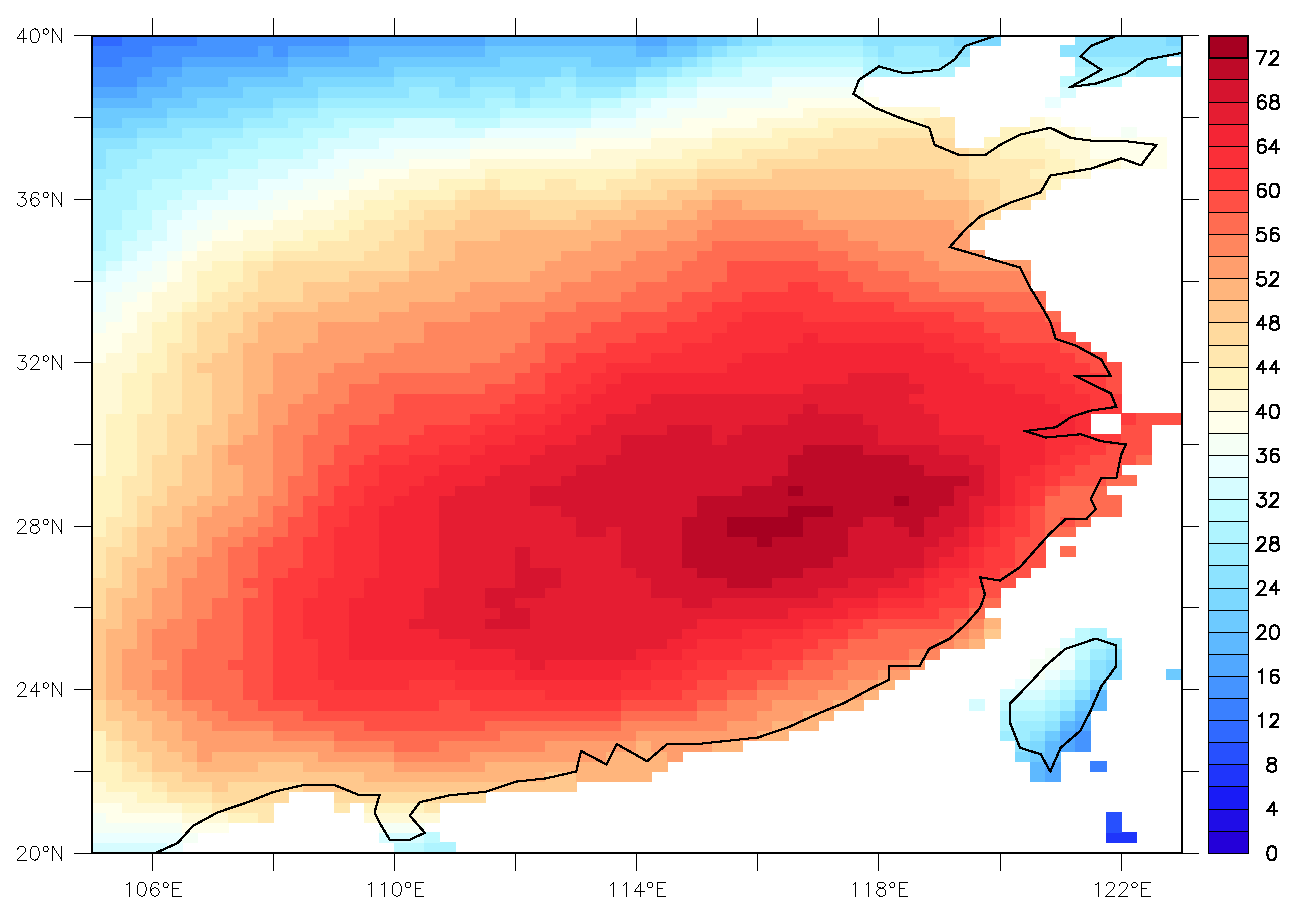
\includegraphics[width=36pc]{Figures/A1_frontpct}
\caption{Percentage of total rainfall at each point in China that is delivered through rainbands (yearly average)}

\label{?}
\end{figure}


\begin{figure}[htb]

\noindent\includegraphics[width=36pc]{Figures/A2_decadal_front}
\caption{1980-2007 versus 1951-1979 changes in frontal and local rainfall for full year (a and b), Pre-Meiyu (c and d) and Post-Meiyu (e and f)}
\end{figure}

\textcolor{red}{In summary, the North Flood-South Drought is describable primarily via changes in banded rainfall. In turn, these changes in banded rainfall are mostly zonally symmetric and coherent across thousands of kilometers, which suggests that they are caused by changes in larger-scale dynamics.}


%% ANDERSON-DARLING AND KOLMOGOROV-SMIRNOV TESTING 
\subsection{Significance of Changes in Rainband Latitude and Intensity Distribution}

We can also test for the statistical significance of the change in the entire distribution, using statistical tests such as the Anderson-Darling test or Kolmogorov-Smirnov test. Each of these tests define test statistics that indicate a confidence estimate that two samples are drawn from the same statistical distribution. The Anderson-Darling test places more weight on outliers relative to the Kolmogorov-Smirnov test, but both are accepted metrics of whether two samples are drawn from the same underlying distribution or not. 

The Kolomogorov-Smirnov test depends first on the definition of the empirical distribution function, equivalent to a statement that each of the observations $X_i$ are weighted evenly in the construction of a cumulative distribution function (CDF):

\begin{align}
	
	F_n(x) &= \frac{1}{n}\sum_{i=1}^n I_{[-\infty,x]} (X_i) \\
	I_{[-\infty,x]} &=
	\begin{cases}
   		 1 & \text{if } X_i \leq x\\
    		0 & \text{otherwise}
    	\end{cases}

\end{align}

While the Anderson-Darling test statistic is defined as:

...

The changes in distribution of latitude and intensity are each shown on separate pages below. In general, the results of the Anderson-Darling and Kolmogorov-Smirnov tests are in agreement with one another, and confirm earlier results. The Pre-Meiyu decline in rainband frequency after 1979 is not reflected in either test, because it is a change in textit{frequency}. On the other hand, the post-Meiyu southward shift in rainband latitude is found to be highly significant by both tests ($p<.001$). No significant changes in rainband intensity are found between 1951-1979 and 1980-2007. Finally, between the time periods 1979-1993 and 1994-2007, a substantial change is found in both the latitude of rainbands during Meiyu season, as well as their intensity when they occur. These tests help to confirm in a statistically rigorous manner that the changes between the time periods 1951-1979 v 1980-2007 and 1979-1993 v 2004-2007 are of a fundamentally distinct character.

%% TABLE 13 - p-value of change in distribution between 1951-1979 and 1980-2007, as calculated by an Anderson-Darling and Kolmogorov-Smirnov test
\begin{table}[p]

\centering

\caption{Statistical significance (express as $p$-value) of change in distribution of latitude and intensity of rainbands between 1951-1979 and 1980-2007, as calculated by both Anderson-Darling and Kolmogorov-Smirnov tests. Statistically significant changes at the 95\%/99\% level are indicated by bold/asterisk and bold.}

\begin{tabular}{ l c c c c}
												& $ \multicolumn{2}{c}{\textbf{Latitude}} $ \multicolumn{2}{c}{\textbf{Intensity}} \\
	 \textbf{Time Period} 							& $\boldsymbol{AD}$ & $\boldsymbol{KS}$ 		& $\boldsymbol{AD}$ & $\boldsymbol{KS}$ \\
	 \hline
	\textbf{Spring Rains} (Mar 1-Apr 30, 60-120)  		& .037			& .086			& .083	& .19 \\
	\textbf{Pre-Meiyu} (May 1-Jun 9, 121-160)  		& .086 			&  .24 			& .90	& .94 \\
	\textbf{Meiyu} (Jun 10-Jul 19, 161-120)			& .21			&  .30			&  .40	& .25 \\	
	\textbf{Post-Meiyu} (Jul 20-Sep 30) 				& \textbf{.0018*}	&  .\textbf{.0073}  	&  .24 	& .28 \\
	\textbf{Post-Meiyu} (Jul 20-Sep 30), $>28^{\circ}N$   & \textbf{.0001*}	&  \textbf{.0010*} 	&  .10 	& .04 \\	
	\textbf{Post-Meiyu} (Jul 20-Sep 30), $<28^{\circ}N$   & .33			&  .38			&  .62	& .53 \\	
	\textbf{Fall Rains} (Oct 1-Nov 16) 					& .15 			&  .23			&  .83 	& .94 \\	
	\textbf{Full Year} (1-365)						& \textbf{.016}	&  .075 			&  .12 	& .26 \\	
	
\end{tabular}
\label{ts13}
\end{table}


%% TABLE 14 - p-value of change in distribution between 1979-1993 and 1994-2007, as calculated by an Anderson-Darling and Kolmogorov-Smirnov test
\begin{table}[p]

\centering

\caption{Statistical significance (express as $p$-value) of change in distribution of latitude and intensity of rainbands between 1979-1993 and 1994-2007, as calculated by both Anderson-Darling and Kolmogorov-Smirnov tests. Statistically significant changes at the 95\%/99\% level are indicated by bold/asterisk and bold.}

\begin{tabular}{ l c c c c}
												& $ \multicolumn{2}{c}{\textbf{Latitude}} $ \multicolumn{2}{c}{\textbf{Intensity}} \\
	 \textbf{Time Period} 							& $\boldsymbol{AD}$ & $\boldsymbol{KS}$ 		& $\boldsymbol{AD}$ & $\boldsymbol{KS}$ \\
	 \hline
	\textbf{Spring Rains} (Mar 1-Apr 30, 60-120)  		& .12			& .34			& .60			& .35 \\
	\textbf{Pre-Meiyu} (May 1-Jun 9, 121-160)  		& .57 			&  .76 			& .29			& .32 \\
	\textbf{Meiyu} (Jun 10-Jul 19, 161-120)			& \textbf{.0002*}	&  \textbf{.0006*}	&  \textbf{.0006*}	& \textbf{.0009*} \\	
	\textbf{Post-Meiyu} (Jul 20-Sep 30) 				& .15			&  .14 			&  .87 			& .48 \\
	\textbf{Post-Meiyu} (Jul 20-Sep 30), $>28^{\circ}N$   & .35			&  .13 			&  .35 			& .26 \\	
	\textbf{Post-Meiyu} (Jul 20-Sep 30), $<28^{\circ}N$   & .60			&  .67			&  .36			& .70 \\	
	\textbf{Fall Rains} (Oct 1-Nov 16) 					& .092 			&  .16			&  .17 			& .40 \\	
	\textbf{Full Year} (1-365)						& .29			&  .14			&  .062 			& .090 \\	
	
\end{tabular}
\label{ts13}
\end{table}

\section{Does the ``South Flood-North Drought'' reflect a jet shift?}

	We also explore decadal changes in the subtropical jet, which plays an essential and complex role in East Asian climate both in summer and winter \citep{Molnar2010,Yang2002}. In a region of strong fronts as observed in East Asia, theory predicts that the core of maximum zonal wind should anchor an equatorward region of ascent and strong rainfall \citep{Holton2004}. The Tibetan Plateau couples with the jet nonlinearly, amplifying the regional response to global climate anomalies \citep{Nigam1989,Broccoli1992,Park1997}. The jet's passage north of the Tibetan Plateau in summer is argued to dictate the timing of onset of the Indian and East Asian monsoons, both in present-day \citep{Yin1949,Yeh1959,Hahn1975} and on paleoclimate timescales \citep{Nagashima2011,Nagashima2013,Chiang2015}. On a weekly timescale, the jet serves as a waveguide for storms propagating from the Eurasian interior via the ``Silk Road'' teleconnection \citep{Hoskins1993,Ambrizzi1997,Kosaka2012}, and shifts in its latitude and strength induce corresponding rainfall anomalies \citep{Liang1998,Kwon2007,Du2009,Li2014}. Thus, we expect that the South Flood-North Drought has also entailed \nth{20}-century changes in the East Asian tropospheric jet. Therefore, we compare our rainband database to a database of jet counts from 1958 to 2001 from \citet{Schiemann2009} in search of coupled change.
	
\subsection{Jet Count Density} 

	\citet{Schiemann2009} constructed a data set of jet `counts' in the Tibetan Plateau region (46$^{\circ}$ E-130\$^{\circ}$ E, 17\$^{\circ}$ N-58\$^{\circ}$ N) from ERA-40 reanalysis for 1958-2001, where a count is defined as any local maximum in zonal wind with westerly magnitude greater than $30$ m s$^{-1}$; further details can be found in section 2 of \citet{Schiemann2009}. We show daily mean jet latitude averaged across $90-130^\circ$E in Figure \ref{jet_seasonal}a and monthly anomalies in Figure \ref{jet_seasonal}b. Results are not sensitive to the choice of longitude range. Figure \ref{climo} presents contours of jet frequency estimated by a kernel density method, which estimates a probability distribution from a set of discrete data observations (Supplementary Text S4).

\subsection{Dynamics}

	The tropospheric jet marks the northern boundary of the Hadley Cell, and shifts in response to seasonal changes in insolation \citep{Bordoni2008}. Beginning in May, the East Asian jet moves from its winter position on the southern flank of the Tibetan Plateau to a summer latitude well north of the plateau. During this transition, the jet occupies intermediate configurations that correspond to different stages of China rainfall (Figure \ref{climo}). A full monthly jet climatology is visible in \citet{Schiemann2009}. Peak rainfall rates in China from May to mid-July corresponds to the months when the climatological latitude of the jet impinges on the Tibetan Plateau. The interaction of the tropospheric jet and Tibetan Plateau strengthens convergence and rainfall downstream over China and the western Pacific Ocean \citep{Molnar2010,Sampe2010,Chen2014}. From May to September,  the climatological latitude of rainfall, rainbands and jet density are all closely coupled, with peak jet density occurring 5 to 10 degrees north of the latitude of peak rainfall. The initiation of the Pre-Meiyu corresponds roughly to the beginning of the jet's northward passage. During Meiyu season, the preferred latitude of the jet continues to shift northward. The period of frequent double rainband occurrence during the Post-Meiyu corresponds to the jet's maximal northward extent. Finally, the jet returns southward during the Fall Rains in October and November, which produces only a weak rainfall response.
	
\subsection{Jet Changes, 1980-2001 Versus 1958-1979}

	In Figure \ref{jet_seasonal}a, we show the zonal average over $90-130^\circ$E) of mean jet latitude, averaged over the years 1958-1979 (blue solid line) and 1980-2001 (dashed red line) with 95\% confidence intervals overlain. Both significant changes in rainband statistics described in the previous section correspond to southward shifts in mean jet latitude. During the Pre-Meiyu (May), the tropospheric jet is shifted southward by almost 2\$^{\circ}$\ in 1980-2001 relative to 1958-1979, when its mean latitude was $\approx 41^\circ$N. We estimate the significance of this change using a two-tailed Kolmogorov-Smirnov (K-S) test. Since the K-S test requires that all samples are independent, we first remove temporal autocorrelation due to synoptic variability by assimilating daily mean jet latitude into 4 day blocks (Supplementary Figure S5). A subsequent K-S test finds that the shift is significant with $p=0.003998$. During the Post-Meiyu (days 201-273), when a southward shift in rainband latitude is found in 1980-2001 relative to 1958-1979, the mean latitude of the jet is also consistently displaced southward. We assimilate daily mean jet latitude into 7-day blocks (Supplementary Figure S5) before performing a K-S test, and find a $p$-value of this shift of $p=0.05667$.

\section{Hypothesis}

	The Meiyu front and tropospheric jet covary in latitude from May to September in the climatological mean, and parallel changes are found in rainband attributes and mean jet latitude between 1951-1979 and 1980-2007. Therefore, the South Flood-North Drought appears to reflect an alteration in jet dynamics. We propose that both the Pre-Meiyu decline in rainband frequency and the Post-Meiyu southward shift of rainband latitude result from a single phenomenon: an overall southward displacement of the jet's summer progression over East Asia. In climatology, the Pre-Meiyu corresponds to both a surge in rainfall and the beginning of the jet's northward transit, when its preferred latitude begins to impinge on the Tibetan Plateau. We propose that the observed southward shift in the jet during May has delayed the date when the jet first impinges on the Tibetan Plateau, resulting in a delay in Pre-Meiyu onset and prolonged Spring Rain conditions. This is manifested as weaker rainfall and decreased rainband frequency in central China in May. Subsequently, we argue that the reduced northward extent of the jet during the Post-Meiyu has shifted rainfall and mean rainband latitude southward. Finally, we suggest that the southward displacement of the summer jet cycle results in a decrease in northern China annual rainfall and an increase in central China annual rainfall, producing a South Flood-North Drought response. Thus, our hypothesis can explain the major observed changes in rainfall and rainband statistics during the Pre- and Post-Meiyu as well as cumulative yearly change.
	
	To test our hypothesis, we investigate the relation of interannual anomalies in jet latitude and rainband properties. Figure \ref{jet_seasonal}b shows a scatter plot of rainband \textit{frequency} anomalies versus jet latitude anomalies in May (days 121-150). Most years with a decrease in rainband frequency feature a southward jet shift, and vice-versa, and such years occur mostly during 1980-2007. A similar relation is found between monthly anomalies in rainband \textit{latitude} and jet latitude during July-August (days 201-260, Figure \ref{jet_seasonal}c). In the latter figure, we exclude rainbands south of 28\$^{\circ}$ N from calculated anomalies, since such rainbands reflect South China Sea storms, rather than jet influence \citep{Day2015}. Together, Figures \ref{jet_seasonal}b and \ref{jet_seasonal}c suggest that interannual changes in jet latitude affect Pre-Meiyu rainband frequency and Post-Meiyu rainband latitude.

	 Observations show that the global annual mean latitude of the tropospheric jet has shifted poleward, in tandem with tropospheric heating and lower-stratospheric cooling in the mid-latitudes, increased subtropical static stability, and the expansion of the Hadley circulation \citep{Fu2006,Archer2008,Fu2011}. Opposite trends are found in some regions and the variation by season is significant; we find that the East Asian portion of the jet has shifted equatorward, in agreement with past studies \citep{Yu2007, Archer2008}. Recent work proposes that the observed southward displacement of the jet over the Pacific Ocean was caused by \nth{20}-century changes in tropical Pacific convection and SST \citep{Park2014a}. Thus, the global poleward trend in jet latitude and the East Asian equatorward shift are compatible observations that reflect the heterogeneous spatial distribution of \nth{20}-century warming.
	 
	 In addition to the late 1970s change in China rainfall, earlier onset of rainfall over the South China Sea during 1994-2008 relative to 1979-1993 has been reported \citep{Kajikawa2012}, as well as an increase in rainfall over southern China and in the passage of tropical cyclones \citep{Kwon2007,Chang2014}. In Supplementary Tables S7 and S8, we find a rise in rainband intensity during Meiyu season (days 161-200) from 27.3 to 29.8 mm day$^{-1}$ ($p=.9994$), and a southward shift in rainband latitude from 30.0\$^{\circ}$ N to 28.9\$^{\circ}$\ N ($p=.0002$). No significant changes are found in rainband frequency or jet latitude. The strengthening and southward shift of Meiyu season rainbands beginning in the mid-1990s merits further investigation.
	 				
\section{Conclusion}

	Using a recursive convergent image processing algorithm, we created an unprecedented database and 57-year climatology of frontal rainfall properties over China, including probability of rainband occurrence and mean latitude, intensity, tilt, width and length. Two statistically significant changes in rainband attributes occurred between the years 1951-1979 and 1980-2007: 1) A decrease in frequency during the Pre-Meiyu season (days 121-160, May 1-June 9; $p=.020$); and 2) A southward shift in latitude of rainbands during the Post-Meiyu season (days 201-273, July 20-Sep 30; $p=.0003$). The latter change is responsible for the South Flood-North Drought trend in total yearly rainfall. During 1994-2007 versus 1979-1993, a substantially different change is found featuring a substantial change in both rainband latitude and intensity during Meiyu season, as quantified by an Anderson-Darling test ($p=.0002$ and $p=.0006$ respectively). Our algorithm shows that 55.6\% of total rainfall falling over China from 1951 to 2007 occurs in rainbands. The development of the rainband detection algorithm allows us to study both frontal rainfall, which is associated with larger-scale variability, and local storms, which may result from meso-scale features such as low mountains, and the distinct changes in each. Each type of rainfall is separately available our data set.
	 
	It is essential to understand whether the South Flood-North Drought will persist under \nth{21}-century warming, or manifests an ephemeral decadal change. However, the CMIP5 (Climate Model Intercomparison Project) model suite contained in the Intergovernmental Panel on Climate Change's Fifth Assessment Report (IPCC AR5) does not agree on the sign of future summer rainfall changes in East Asia \citep{Christensen2011}. In this study, we have found robust changes in frontal rainfall. The poleward expansion of the Hadley Cell is projected to continue under \nth{21}-century warming \citep{Lu2007,Kang2012}, but a recent study predicts that anomalous \nth{21}-century heating of the eastern Pacific Ocean will drive the Pacific jet further equatorward \citep{Park2014}. By linking the South Flood-North Drought to changes in the seasonal advance of the tropospheric jet, we open the possibility of projecting \nth{21}-century East Asian rainfall change by improving our understanding of the effect of further global warming on the regional and global behavior of the tropospheric jet.
	
	Many components of our results have been presented in previous work. \citet{Xuan2011} find a southward shift in the jet and increased Yangtze Valley rainfall in July. \citet{Yu2004} and \citet{Yu2007} found a southward shift in July-August jet latitude and suggested a link with the South Flood-North Drought. Potential mechanisms for late \nth{20}-century East Asian climate change include changes in Indian Ocean SST \citep{Qu2012}, decreased sensible heating from the Tibetan Plateau \citep{Liu2012a,Hu2015} and aerosol forcing \citep{Song2014}. Other studies attribute the South Flood-North Drought to natural variability \citep{Zhang1999,Xin2006,Lei2014}, but \citet{Zhou2009} claimed that the South Flood-North Drought was distinct from other patterns of \nth{20}-century variability. 


\section{Acknowledgments}

	APHRODITE precipitation data is publicly available at \url{http://www.chikyu.ac.jp/precip/index.html}. Ferret, a NOAA product, was used for some data analysis and preliminary plot generation and is freely available at \url{http://ferret.pmel.noaa.gov/Ferret/}. The rainband detection algorithm and the majority of data analysis code were written in MATLAB. A full database of rainband statistics from 1 January 1951 to 31 December 2007 and associated MATLAB and Ferret codes used to produce results are available at the author's website: \url{http://www.atmos.berkeley.edu/~jessed/data.html}, and key figures are reproduced at \url{http://www.atmos.berkeley.edu/~jessed/myfigures.html}. This work was supported by NSF grants EAR-0909195 and EAR-1211925, which allowed the presentation of preliminary results in conference settings and the feedback of our peers. We also acknowledge NSFC (National Natural Science Foundation of China) grant \#40921120406 for enabling our collaboration with Professor Yanjun Cai of IEECAS in Xi'an, which led to the present work. We thank Jinqiang Chen and an anonymous reviewer for valuable suggestions for a prior version of the present manuscript.
